\documentclass[11pt,a4paper,twocolumn]{article}

% === Core Packages ===
\usepackage[margin=2cm]{geometry}
\usepackage[utf8]{inputenc}
\usepackage[T1]{fontenc}
\usepackage{times}
\usepackage{amsmath,amssymb}
\usepackage{graphicx}
\usepackage{booktabs}
\usepackage{float}
\usepackage{enumitem}
\usepackage{tikz}
\usepackage{pgfplots}
\pgfplotsset{compat=1.18}
\usetikzlibrary{arrows.meta,shapes.geometric,positioning,calc,decorations.markings,fit,backgrounds}

% === Citation (IEEE style) ===
\usepackage[numbers,sort&compress]{natbib}
\bibliographystyle{IEEEtranN}

% === Hyperref ===
\usepackage[hidelinks]{hyperref}
\usepackage{xurl}

% === Settings ===
\setlength{\parindent}{1em}
\setlength{\parskip}{0.3em}

% === Title ===
\title{\textbf{Detsentraliseeritud reputatsioonivõrk:\\Raamistik ühiskonna loomulikuks korralduseks}}
\author{Pavel Kudrna\\Praha, Tšehhi\\Mustand v1 --- märts 2026}
\date{}

\begin{document}
\maketitle

% ============================================================
% ABSTRACT
% ============================================================
\begin{abstract}
Õiglustunne---veendumus, et ülekohus heastatakse ja teened saavad tasu---on ühiskonna tugevaim ühendav jõud. Kui tsentraliseeritud valitsemisinstitutsioonid ei suuda seda tunnet pakkuda, sest õiguse jõustamise kulu ületab õiguse enda väärtuse, siis sotsiaalne sidusus mureneb. Praegused institutsionaalsed struktuurid ei suuda lahendada olulist osa vaidlustest süstemaatiliselt samamoodi, nagu tsentraalne planeerimine ei suuda ressursse jaotada: infoasümmeetria, puuduvate tagasisidesilmuste ning otsustajate lahutatuse tõttu oma otsuste tagajärgedest. See artikkel esitab reputatsiooni-suhtlusvõrgustiku (Reputation Social Network, RSN): detsentraliseeritud, korrumpeerimatu ja tsensuurikindla suhtluskihi, mis on ehitatud detsentraliseeritud identifikaatoritele (Decentralized Identifiers, DID) ja mis võimaldab pseudonüümsetel osalejatel avaldada, kontrollida ja tarbida reputatsiooniteavet reaalse maailma käitumise kohta. Põhimehhanism tugineb kolmele projekteerimispõhimõttele: (1)~asümmeetriline kulustruktuur, kus reputatsiooniandmete lugemine on odav, kuid kirjutamine nõuab kontrollitavat pingutust; (2)~mittedeterministlik kontrollijate valimise protokoll, mis põhineb järjepideval räsimisel (consistent hashing) ja hinnastab radikaalsed väited kasvavate iteratsioonikulude kaudu; ning (3)~turupõhine reputatsiooniautoriteedi mudel, kus eraviisilised kontrollijad panevad oma kogunenud reputatsiooni kaalule nende väidete täpsuse eest, mida nad kinnitavad. Sellest tulenev arhitektuur loob esilekerkiva meritokraatia ilma tsentraalse koordineerimiseta ning võimaldab järkjärgulist ja pöörduvat üleminekuteed olemasolevatelt riigi hallatavatelt süsteemidelt.
\end{abstract}

% ============================================================
% 1. INTRODUCTION
% ============================================================
\section{Sissejuhatus}

\subsection{Tsentraliseeritud usalduse probleem}

Kaasaegne valitsemine tugineb ühele põhimõttelisele eeldusele: et tsentraliseeritud institutsioonid suudavad vahendada usaldust võõraste vahel suures mastaabis. Kohtud lahendavad vaidlusi. Registrid tõendavad omandit. Reguleerivad asutused jõustavad standardeid. Need institutsioonid loodi ajastul, mil teave oli napp, suhtlus aeglane ning võimu delegeerimine tsentraalsele organile oli ainus teostatav koordineerimismehhanism. Tsentraliseeritud valitsemine aga ebaõnnestub samadel struktuurilistel põhjustel nagu tsentraalne planeerimine: infoasümmeetria, puuduvad tagasisidesilmused ning otsustajate lahutatus oma otsuste tagajärgedest.

See eeldus ebaõnnestub näiteks siis, kui institutsionaalse vahendamise kulu ületab vaidluse väärtuse. Vaatleme üürnikku, kes avastab, et tema üüritud korteril puudub seaduslikult nõutav elektriohutuse tunnistus---seisund, mis kujutab endast vahetut ohtu elule. Üürniku seaduslik õigus lepingust taganeda on ühemõtteline. Ometi ületab selle õiguse jõustamise kulu kohtusüsteemi kaudu tagatisraha ja hüvitatava kahju rahalise väärtuse, isegi arvestades võimalikku seadusjärgset kompensatsiooni~\cite{czcourtfees}. Ratsionaalne vastus on kahju kanda ja lahkuda.

See ei ole patoloogiline erandjuhtum. See on vaikimisi kogemus olulise klassi vaidluste puhul, kus kahju on reaalne, kuid rahaline panus jääb allapoole künnist, mille juures institutsionaalne jõustamine muutub majanduslikult ratsionaalseks. Tulemuseks on süsteem, mis struktuurilt soosib pahatahtlikke tegutsejaid: need, kes kahjustavad teisi selle künnise alla jäävates mahtudes, saavad tegutseda karistamatult, sest õiguse otsimise kulu langeb kahjustatud poolele.

Ülaltoodud näide pärineb autori õiguskeskkonnast---Tšehhi tsiviilõigussüsteemist. Teistes õigustraditsioonides---pretsedendipõhises üldõiguses, tavaõiguses, segasüsteemides---ebaõnnestub õiglus erineval viisil ja erineval määral sõltuvalt jurisdiktsiooni kultuurilistest ja menetluslikest eripäradest. Lugejad tunnevad tõenäoliselt ära samaväärseid näiteid oma kontekstist. Struktuuriliselt universaalne on muster: vaidlused, mille väärtus jääb allapoole majanduslikult ratsionaalse jõustamise künnist, lõppevad sellega, et kahju kannab kahjustatud pool. RSN ei luba täiuslikku õiglust---see üksnes vähendab struktuurilist eelist, mida pahatahtlikud tegutsejad naudivad siis, kui institutsionaalne jõustamine on ebaökonoomne.

\subsection{Miks olemasolevad lahendused ei ole piisavad}

\textbf{Detsentraliseeritud identiteedi (DID) raamistikud}~\cite{did2022} pakuvad krüptograafilisi mehhanisme iseseisvaks identiteedihalduseks, kuid keskenduvad peamiselt identiteedi kontrollimisele, käsitlemata laiemat käitumusliku reputatsiooni küsimust.

\textbf{Hingega seotud märgid (Soulbound Tokens, SBT)}~\cite{weyl2022} tabavad tõdemuse, et reputatsioon ei ole ülekantav, kuid tuginevad plokiahela taristule koos skaleeritavuse piirangutega ega käsitle teabe sisestamist reguleerivaid majanduslikke stiimuleid. Sarnased kontseptsioonid, nagu teenete märgid (nt Liberland), jagavad sarnast filosoofiat, kuid jäävad seotuks konkreetsete jurisdiktsiooniliste raamistikega.

\textbf{Detsentraliseeritud autonoomsed organisatsioonid (DAO)}~\cite{buterin2014} rakendavad valitsemist nutilepingute kaudu, kuid taastoodavad plutokraatlikku dünaamikat, kus mõjuvõim on proportsionaalne kapitaliga. Ruuthääletus~\cite{buterin2019} leevendab seda osaliselt, kuid piirab praktilist kasutuselevõttu. DAO-d seisavad silmitsi ka põhimõttelise \emph{oraakliprobleemiga}: nutilepingud ei suuda usaldusväärselt kontrollida reaalse maailma seisundeid ilma usaldusväärse välise allikata ning sellel probleemil pole plokiahela arhitektuuri sees üldist lahendust.

Ükski olemasolev süsteem ei ühenda detsentraliseeritust, tsensuurikindlust, pseudonüümsust, kontrollitavat sisenemiskulu ja esilekerkivat konsensust.

\subsection{Panus}

See artikkel annab järgmise panuse:
\begin{enumerate}[nosep]
\item \textbf{Reputatsiooni-suhtlusvõrgustiku (RSN)} määratlus---detsentraliseeritud protokoll, mis laiendab DID-raamistikku kahepoolse reputatsioonivahetuse toetamiseks.
\item \textbf{Mittedeterministlik kontrollijate valimise protokoll}, mis põhineb järjepideval räsimisel~\cite{karger1997}.
\item \textbf{Kalli radikalismi põhimõte}, mis hinnastab väited vastavalt nende kaugusele võrgu konsensusest kolme liituva kulukanali kaudu.
\item \textbf{Reputeeritud autoriteedi mudel} asümmeetriliste stiimulitega, kus vale kinnitamine maksab katastroofiliselt rohkem kui õiguspärane tasu.
\item \textbf{Järkjärguline üleminekutee} paralleelse fiskaaltaristu kaudu.
\end{enumerate}

% ============================================================
% 2. DESIGN PRINCIPLES
% ============================================================
\section{Projekteerimispõhimõtted}

RSN-i arhitektuur on piiratud viie läbiräägitamatu projekteerimispõhimõttega.

\textbf{Järjepidevus ja areng.} Süsteem eksisteerib koos olemasolevate institutsioonidega määramata pikkusega üleminekuperioodil. Üleminek peab olema pöörduv igas etapis.

\textbf{Vabatahtlikkus ja vastutus.} Osalemine on vabatahtlik, kuid vabatahtlikkus on seotud vastutusega: osaleja, kes võtab enda kanda institutsionaalse funktsiooni juhtimise, võtab samaaegselt enda kanda ka sellega kaasnevad kohustused.

\textbf{Mitmekesisus ja kultuuriline neutraalsus.} Konsensus kerkib esile kahepoolsetest interaktsioonidest, mitte süsteemi loojate seatud etteantud reeglitest.

\textbf{Vastupidavus ja tsensuurikindlus.} Võrgu tsenseerimise kulu peab ületama selle sallimise kulu. Ainult täielik totalitarism---laostava poliitilise ja majandusliku hinnaga---suudab süsteemi maha suruda.

\textbf{Konsensus ja jõustamine.} Süsteem hõlmab inimlikke kalduvusi väiklusele, kiusule ja kättemaksurahuldusele kandvate elementidena. Üleastumine ei ole keelatud; see on hinnastatud.

% ============================================================
% 3. SYSTEM OVERVIEW
% ============================================================
\section{Süsteemi ülevaade}

\subsection{Reputatsiooni-suhtlusvõrgustik}

RSN on detsentraliseeritud, otspunktist otspunkti suhtluskiht, milles osalejad vahetavad kontrollitavat teavet reaalse maailma käitumise kohta. Selle määravad omadused on: detsentraliseeritud ja tsenseerimatu taristu; pseudonüümne osalemine DID-ide kaudu; asümmeetriline kulustruktuur (lugemine on odav, kirjutamine kallis); krüptograafiline kontrollitavus; ja \textbf{standardite tugi}---masinloetavad vormingud võrgu kaudu levitatavale teabele, autoriteetide pakutavatele teenustele (väite koostamine, kinnitamine, tunnistajateenus) ning poliitikavormingule, mis hõlmab reegleid vastaspoole reputatsiooni hindamiseks ja poliitika mittevastavuse riski (deklareeritud ja tegeliku käitumise vahel) hindamiseks.

\subsection{Arhitektuurikomponendid}

RSN koosneb neljast põhikomponendist (joonis~\ref{fig:architecture}):
\begin{enumerate}[nosep]
\item \textbf{DID-kiht.} Osalejate identiteedid koos deklareeritud reeglite, reputatsiooni metaandmete ja võrgu marsruutimisega.
\item \textbf{Väiteprotokoll.} Struktureeritud vorming väidete avaldamiseks reaalse maailma sündmuste kohta.
\item \textbf{Kontrollivõrk.} Detsentraliseeritud protokoll kontrollijate määramiseks järjepideva räsimise abil.
\item \textbf{Reputatsiooni koondamise kiht.} Teenused, mis loovad inimloetavaid reputatsioonikokkuvõtteid.
\end{enumerate}

\begin{figure}[ht]
\centering
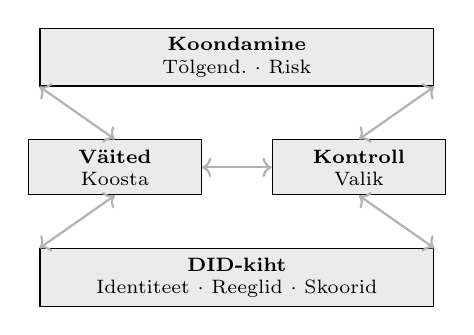
\begin{tikzpicture}[
    layer/.style={draw, minimum height=0.7cm, align=center, font=\scriptsize, fill=black!8},
    arr/.style={<->, thick, gray!60}
]
\node[layer, minimum width=5cm] (agg) at (0,2.8) {\textbf{Koondamine}\\Tõlgend.\ $\cdot$ Risk};
\node[layer, minimum width=2.2cm] (claim) at (-1.55,1.4) {\textbf{Väited}\\Koosta};
\node[layer, minimum width=2.2cm] (verif) at (1.55,1.4) {\textbf{Kontroll}\\Valik};
\node[layer, minimum width=5cm] (did) at (0,0) {\textbf{DID-kiht}\\Identiteet $\cdot$ Reeglid $\cdot$ Skoorid};

\draw[arr] (agg.south west) -- (claim.north);
\draw[arr] (agg.south east) -- (verif.north);
\draw[arr] (claim.east) -- (verif.west);
\draw[arr] (claim.south) -- (did.north west);
\draw[arr] (verif.south) -- (did.north east);
\end{tikzpicture}
\caption{RSN-i neljakihiline arhitektuur.}
\label{fig:architecture}
\end{figure}

\subsection{Osalejate rollid}

Kontrollitehing hõlmab kuni kuut eraldiseisvat DID-rolli (joonis~\ref{fig:roles}): \textbf{Väljaandja} ($DID_I$, loob ja esitab väite), \textbf{Subjekt} ($DID_S$, DID, mille kohta väide käib---võib kattuda Väljaandjaga), \textbf{Autoriteet} ($DID_A$, kinnitab väite tasu eest; võib pakkuda ka tunnistajateenuseid---\emph{valikuline}), \textbf{Tunnistaja} ($DID_{W_{1..n}}$, kontrollija aususe inkognito jälgija väljakutsekoodide abil---\emph{valikuline}), \textbf{Kontrollija} ($DID_V$, algoritmiliselt valitud väidet avaldama) ja \textbf{RSN} (võrk, kus kontrollitud väited avaldatakse). Iga roll võib olla delegeeritud teisele DID-ile (jaotis~7.4). Autoriteet komplekteerib kinnitamise sageli koos tunnistajateenustega, kuid need kaks funktsiooni on loogiliselt sõltumatud.

\begin{figure}[ht]
\centering
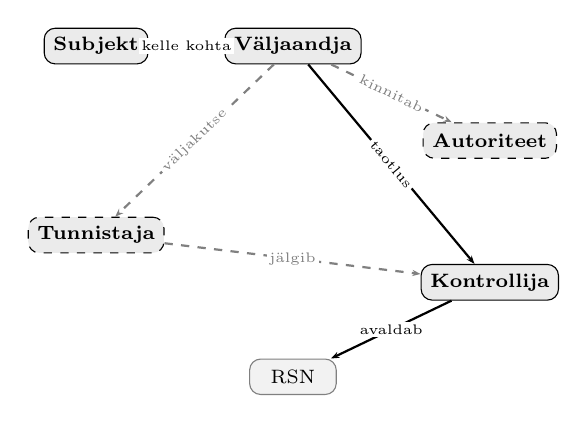
\begin{tikzpicture}[
    role/.style={draw, rounded corners, minimum width=1.1cm, minimum height=0.45cm, align=center, font=\scriptsize, fill=black!8},
    opt/.style={draw, rounded corners, minimum width=1.1cm, minimum height=0.45cm, align=center, font=\scriptsize, fill=black!8, dashed},
    arr/.style={-{Stealth[length=3pt]}, thick},
    oarr/.style={-{Stealth[length=3pt]}, thick, dashed, gray},
    lbl/.style={font=\tiny, fill=white, inner sep=1pt}
]
\node[role] (I) at (0,2.4) {\textbf{Väljaandja}};
\node[role] (S) at (-2.5,2.4) {\textbf{Subjekt}};
\node[opt] (A) at (2.5,1.2) {\textbf{Autoriteet}};
\node[opt] (W) at (-2.5,0) {\textbf{Tunnistaja}};
\node[role] (V) at (2.5,-0.6) {\textbf{Kontrollija}};
\node[role, fill=black!5, draw=gray] (N) at (0,-1.8) {RSN};

\draw[arr] (I) -- node[lbl] {kelle kohta} (S);
\draw[oarr] (I) -- node[lbl,sloped] {kinnitab} (A);
\draw[oarr] (I) -- node[lbl,sloped] {väljakutse} (W);
\draw[arr] (I) -- node[lbl,sloped] {taotlus} (V);
\draw[oarr] (W) -- node[lbl] {jälgib} (V);
\draw[arr] (V) -- node[lbl] {avaldab} (N);
\end{tikzpicture}
\caption{DID-rollid kontrollitehingus. Katkendjoon = valikuline (Autoriteet, Tunnistaja).}
\label{fig:roles}
\end{figure}

\subsection{Korrumpeerimatus: neli jõudu}

RSN-i korrumpeerimatus ei tulene ühest mehhanismist, vaid neljast samaaegsest jõust. Ükski neist ei ole iseseisvalt piisav; ainult nende kombinatsioon muudab korruptsioonikatse majanduslikult ebaratsionaalseks.

\textbf{Ettearvamatu sihtmärk.} Iga väite kontrollija valitakse mittedeterministlikult järjepideva räsimise abil (jaotis~5.3). Ründaja ei saa konkreetset kontrollijat altkäemaksuks ette sihikule võtta, sest kontrollija identiteet on väite sisu ja varasemate iteratsioonide funktsioon, mitte väljaandja valik.

\textbf{Reputatsiooni võimendus---aeglaselt üles, kiiresti alla.} Reputatsiooni saab omandada üksnes järk-järgult, püsiva järjepideva käitumise kaudu. Selle võib aga katastroofiliselt kaotada ühe pettusliku kinnitamisega (jaotis~6.2). See asümmeetria tähendab, et aastatega kogunenud reputatsiooni võib hävitada üksainus ebaaus kinnitamine; optimaalseks strateegiaks jääb kahtlaste väidete tagasilükkamine.

\textbf{Avalik lubadus.} Iga DID-i valdaja deklareerib avalikult oma poliitika---masinloetava reeglistiku, mida ta kohustub järgima. Lahknevus deklaratsiooni ja tegeliku käitumise vahel on tuvastatav ja hinnastatud reputatsioonirikkumisena, mis on raskem kui aluseks olev rikkumine ise (jaotis~7.3). Silmakirjalikkus on seega kulukam kui otsene ebaausus.

\textbf{Võrgustiku ründekulu asümmeetria.} Võrgu tsenseerimise või destabiliseerimise kulu kasvab mittelineaarselt koos võrgu suuruse ja tihedusega, samas kui selle sallimise kulu jääb konstantseks. Et tsensuur end ära tasuks, peaks tsentraliseeritud tegutseja rakendama seda kogu võrgu ulatuses---nõudes meetmeid, mis on ebaproportsionaalsed igasuguse kujuteldava kasuga (jaotis~10).

% ============================================================
% 4. DECENTRALIZED IDENTITY MODEL
% ============================================================
\section{Detsentraliseeritud identiteedi mudel}

\subsection{DID eriomadustega}

RSN laiendab W3C DID Core spetsifikatsiooni~\cite{did2022} järgmisega: \textbf{Deklareeritud reeglid} (masinloetavad käitumuslikud kohustused), \textbf{Reputatsiooni metaandmed} (koondatud käitumuslik skoor) ja \textbf{Võrgu marsruutimine} (muudetav sibulavärav, eraldi stabiilsest ringiasendist).

\subsection{Väite elutsükkel}

Väide läbib kuus etappi (joonis~\ref{fig:lifecycle}): koostamine, valikuline autoriteedi kinnitamine, kontrollija valimine järjepideva räsimise abil, kontrollimisotsus (heakskiit või tagasilükkamine koos iteratsiooniga), avaldamine ja reputatsiooni uuendamine kõigi osapoolte jaoks.

\begin{figure}[ht]
\centering
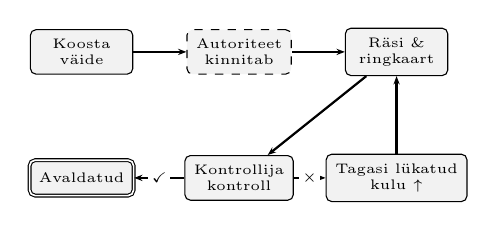
\begin{tikzpicture}[
    stp/.style={draw, rounded corners=2pt, minimum width=1.3cm, minimum height=0.45cm, align=center, font=\tiny, fill=black!5},
    arr/.style={-{Stealth[length=3pt]}, thick},
    lbl/.style={font=\tiny, fill=white, inner sep=1pt}
]
\node[stp] (comp) at (0,0) {Koosta\\väide};
\node[stp, dashed] (auth) at (2.0,0) {Autoriteet\\kinnitab};
\node[stp] (hash) at (4.0,0) {Räsi \&\\ringkaart};
\node[stp] (ver) at (2.0,-1.6) {Kontrollija\\kontroll};
\node[stp, double] (pub) at (0,-1.6) {Avaldatud};
\node[stp] (rej) at (4.0,-1.6) {Tagasi lükatud\\kulu $\uparrow$};

\draw[arr] (comp) -- (auth);
\draw[arr] (auth) -- (hash);
\draw[arr] (hash) -- (ver);
\draw[arr] (ver) -- node[lbl] {\checkmark} (pub);
\draw[arr] (ver) -- node[lbl] {$\times$} (rej);
\draw[arr] (rej) -- ++(0,0.8) -| (hash);
\end{tikzpicture}
\caption{Väite elutsükkel koos iteratsioonisilmusega.}
\label{fig:lifecycle}
\end{figure}

\subsection{Suhe W3C DID Core'iga}

RSN-i identiteedimudel on W3C DID Core spetsifikatsiooni~\cite{did2022} korrektne ülemhulk. Kõik RSN-i DID-id on kehtivad W3C DID-id. RSN-spetsiifilised laiendused on kodeeritud DID-dokumendi omadustena, mis on määratletud spetsiaalses DID-meetodi spetsifikatsioonis, ühilduvana olemasoleva taristuga nagu ION~\cite{buchner2021} ja Ceramic~\cite{ceramic2023}.

% ============================================================
% 5. VERIFICATION AND PROPAGATION
% ============================================================
\section{Teabe kontrollimine ja levitamine}

\subsection{Teabe sisestamise kulu}

RSN-i keskne majanduslik põhimõte on asümmeetria lugemise ja kirjutamise vahel. Reputatsiooniandmete lugemine läheneb nullilähedasele piirkulule osalejate jaoks, kes on osa DID-võrgust ja kellel on nende reputatsioonile vastav juurdepääs---uustulnukad peavad järk-järgult teenima laiema juurdepääsu (vt parasiitluse tõkestamine). Kirjutamine---mõistetuna kui reputatsiooni püsiv materialiseerumine võrku, mitte kui ühekordne tehniline akt---nõuab kontrollitavat kumulatiivset investeeringut kolmes mõõtmes: \textbf{aeg} (järjepidevale käitumisele, täidetud kohustustele ja kultiveeritud suhetele kulutatud eluaastad), \textbf{energia} (ausasse tegutsemisse, partnerlussuhete hoidmisse ja pikaajalisse usaldusväärsusesse investeeritud pingutus) ja \textbf{raha} (investeering oma nimesse---erialane areng, oma töö kvaliteet, tekitatud kahjude hüvitamine). Reputatsiooni ei saa hetkega osta---see on eluaegse kogunemise tulemus, mille süsteem üksnes muudab nähtavaks ja kontekstideüleselt ülekantavaks. Protokolli ühekordsed tehnilised kulud (krüptograafilised allkirjad, kontrollijatasud) on selle aluseks oleva investeeringuga võrreldes tühised.

\subsection{Sotsiaalne graaf ja kontaktide sügavus}

RSN on olemuslikult sotsiaalne võrgustik: iga DID lisab kontakte (teisi DID-e), kes ühenduse lubavad. Neil kontaktidel on oma kontaktid ja nii edasi. Algoritmiline kontrollijate otsing toimib seotud kontaktide seadistatava sügavuse $h$ piires (nt $h=3$: enda otsekontaktid, nende kontaktid ja kontaktide kontaktid). See arhitektuur ei nõua ühte globaalset plokiahelat---see soosib loomulikult kogukondade/klastrite esilekerkimist koos kattumistega teistesse kogukondadesse. Igal DID-osalejal peab olema avaldatud \textbf{poliitika}---masinloetav reeglistik, mis reguleerib, kuidas sissetulevaid taotlusi hinnatakse. Poliitika rikkumised salvestatakse võrku negatiivsete artefaktidena.

\subsection{Algoritmiline kontrollijate valimine}

Kontrolliprotokoll kasutab järjepidevat räsimist~\cite{karger1997} (joonis~\ref{fig:verifier}). Kontrollimine on tasuline teenus: kontrollijad tegutsevad tasu eest, luues turu, kus konkurents suunab hinnastamist, kiirust ja usaldusväärsust.

\textbf{Samm 1.} Väitedokument liidetakse eelmise iteratsiooni räsitulemusega (või $\varnothing$ esimesel iteratsioonil) ja räsitakse:
\begin{equation}
\text{pos} = f_h(\text{claim} \| \text{prev\_hash})
\label{eq:hash}
\end{equation}

Algoritm peab hõlmama kõigi varasemate taotluste ja vastuste \emph{täieliku tee}---mitte üksnes eelmise iteratsiooni räsi. Iga kontrollija täielik vastus (heakskiit, tagasilükkamine, pakutud hind, põhjus) lisatakse kasvavale dokumendile, mis on kontrollitav krüptograafiliste allkirjade abil igas etapis.

\textbf{Samm 2.} Räsi kaardistatakse $N$ asendile järjepideva räsiringi peal, ühtlaselt jaotatuna (nt $N=4$ korral: $+0^{\circ}, +90^{\circ}, +180^{\circ}, +270^{\circ}$). Igast asendist valib päripäeva otsing lähima DID-i kontrollijakandidaadiks (joonis~\ref{fig:multipoint}). $N$ on muutuv parameeter, mis võib sõltuda hetkel aktiivsete DID-ide protsendist, kellaajast või võrgu ajaloolisest reageerimiskiirusest.

\textbf{Samm 3.} Kontrollija kas nõustub (avaldab, pannes reputatsiooni kaalule) või lükkab tagasi (naastes sammu~1 juurde tagasilükkamise räsiga). Kui sõlm ei reageeri hoolimata veebis-oleku deklareerimisest, peab järgmine taotlus sisaldama kõiki vastuseid kõigilt $N$ varasemalt kontrollijakandidaadilt.

\textbf{Parasiitluse tõkestamine.} Siht-DID-id võivad seada tasud või juurdepääsupiirangud vähese reputatsiooniga uute DID-ide päringutele. See astmeline mehhanism (mitte binaarne) sunnib uustulnukaid ehitama reputatsiooni ehtsa tegevuse kaudu, enne kui nad saavad vabalt teiste andmeid tarbida.

\begin{figure}[ht]
\centering
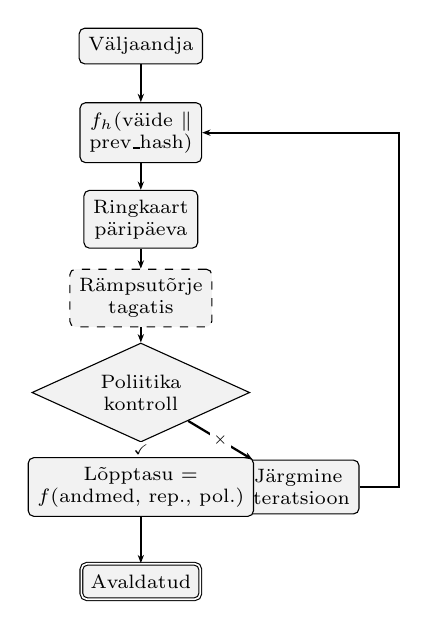
\begin{tikzpicture}[
    box/.style={draw, rounded corners=2pt, minimum width=1.3cm, minimum height=0.45cm, align=center, font=\scriptsize, fill=black!5},
    dec/.style={draw, diamond, aspect=2.2, minimum width=0.9cm, align=center, font=\scriptsize, fill=black!5},
    arr/.style={-{Stealth[length=3pt]}, thick},
    lbl/.style={font=\tiny, fill=white, inner sep=1pt}
]
\node[box] (iss) at (0,0) {Väljaandja};
\node[box] (hash) at (0,-1.1) {$f_h$(väide $\|$\\prev\_hash)};
\node[box] (ring) at (0,-2.2) {Ringkaart\\päripäeva};
\node[box, dashed] (spam) at (0,-3.2) {Rämpsutõrje\\tagatis};
\node[dec] (check) at (0,-4.4) {Poliitika\\kontroll};
\node[box] (rej) at (2,-5.6) {Järgmine\\iteratsioon};
\node[box] (fee) at (0,-5.6) {Lõpptasu =\\$f$(andmed, rep., pol.)};
\node[box, double] (pub) at (0,-6.8) {Avaldatud};

\draw[arr] (iss) -- (hash);
\draw[arr] (hash) -- (ring);
\draw[arr] (ring) -- (spam);
\draw[arr] (spam) -- (check);
\draw[arr] (check) -- node[lbl] {$\times$} (rej);
\draw[arr] (check) -- node[lbl] {\checkmark} (fee);
\draw[arr] (fee) -- (pub);
\draw[arr] (rej.east) -- ++(0.5,0) |- (hash.east);
\end{tikzpicture}
\caption{Kontrollija valimise protokoll. Rämpsutõrje tagatis on valikuline ja võib olla tagastatav. Lõpptasu makstakse ainult heakskiidu korral.}
\label{fig:verifier}
\end{figure}

Iga tagasilükkamine lisab väitedokumendile kontrollija täieliku vastuse (kaasa arvatud põhjused ja tingimused), laiendades selle sisu. Laiendatud dokumendist arvutatakse mittedeterministlikult uus räsi, mis kaardistub teisele ringiasendile ja valib teise kontrollija. Täieliku tee dokumenteerimine on kohustuslik---väljaandja ei saa järgmist kontrollijat ennustada ega mõjutada. Kui kontrollija ignoreerib taotlust hoolimata ühilduvast deklareeritud poliitikast, salvestavad tunnistajad (kui neid on) selle ning väljaandja võib lõplikul avaldamisel lisada tunnistaja tõendid.

\begin{figure}[ht]
\centering
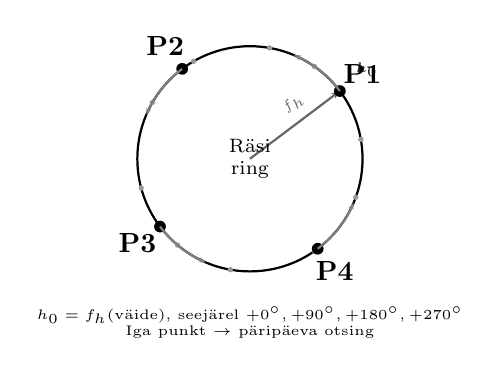
\begin{tikzpicture}[scale=0.65]
% Ring
\draw[thick] (0,0) circle (2.2cm);
% DID nodes on ring
\foreach \a in {10,55,80,120,150,195,230,260,305,340} {
  \fill[black!40] (\a:2.2) circle (1.5pt);
}
% Hash offset arrow pointing to initial position
\draw[-{Stealth[length=3pt]}, thick, black!60] (0,0) -- node[font=\tiny,above,sloped,pos=0.6] {$f_h$} (37:2.2);
\fill[black] (37:2.2) circle (2pt);
\node[font=\tiny,anchor=south west] at (37:2.35) {$h_0$};
% N=4 points offset from h0 by +0, +90, +180, +270
\foreach \offset/\l in {0/P1,90/P2,180/P3,270/P4} {
  \pgfmathsetmacro{\ang}{37+\offset}
  \node[fill=black, circle, inner sep=1.5pt] (p\offset) at (\ang:2.2) {};
  \node[font=\tiny,font=\bfseries] at (\ang:2.75) {\l};
  % clockwise search arc
  \draw[-{Stealth[length=2.5pt]}, thick, gray] (\ang:2.2) arc (\ang:\ang+30:2.2);
}
\node[font=\scriptsize, align=center] at (0,0) {Räsi\\ring};
\node[font=\tiny, align=center] at (0,-3.2) {$h_0 = f_h(\text{väide})$, seejärel $+0^{\circ},+90^{\circ},+180^{\circ},+270^{\circ}$\\Iga punkt $\rightarrow$ päripäeva otsing};
\end{tikzpicture}
\caption{Mitmepunktiline valik ($N{=}4$). Räsi $h_0$ määrab nihke; 4 punkti ühtlaselt jaotatud alates $h_0$.}
\label{fig:multipoint}
\end{figure}

\subsection{Tunnistajaprotokoll}

\textbf{Tunnistaja} roll pakub inkognito vastutust kontrollija aususe eest krüptograafilise väljakutsekoodi protokolli kaudu:

\textbf{Samm W1.} Taotleja allkirjastab kontrollitaotluse ja saadab selle $N_w$ tunnistajale---taotleja sotsiaalvõrgustiku kontaktid või spetsialiseeritud tunnistajateenuse pakkujad, kes tegutsevad tasu eest.

\textbf{Samm W2.} Iga tunnistaja $w_i$ allkirjastab kogu allkirjastatud taotluse, säilitab originaalallkirja $\sigma_i$ ja arvutab väljakutsekoodi $c_i = h(\sigma_i)$. Väljakutsekood lisatakse taotlusele.

\textbf{Samm W3.} Taotlus, mis nüüd kannab $N_w$ väljakutsekoodi, saadetakse kontrollijale. Kontrollija näeb koode, kuid \emph{ei suuda kindlaks teha}, kes on tunnistajad ega kas koodid vastavad tegelikele allkirjadele.

\textbf{Samm W4 (aus kontrollija).} Kui kontrollija reageerib vastavalt oma deklareeritud poliitikale, jäävad väljakutsekoodid läbipaistmatuks. Tunnistajaid ei avalikustata kunagi. Täiendavaid andmeid ei avaldata.

\textbf{Samm W5 (poliitika rikkumine).} Kui kontrollija rikub oma poliitikat (ignoreerib taotlust, reageerib ebajärjekindlalt), hoiab taotleja tunnistajate originaalallkirju $\sigma_i$. Need saab avaldada kaasandmetena: igaüks saab kontrollida, et $c_i = h(\sigma_i)$, tõestades, et tunnistaja oli kohal. Taotleja saab avaldada iseseisvalt---kontrollija on väljakutsekoodid oma vastuses juba allkirjastanud.

\textbf{Blufi omadus.} Taotleja võib asendada mõned või kõik väljakutsekoodid juhuslike väärtustega. Kontrollija ei suuda eristada ehtsaid koode (mida toetavad kõrge reputatsiooniga autoriteedid) mürast. See \emph{ebakindlus} on jõustamismehhanism: iga taotlus kannab riski, et austusväärne autoriteet jälgib inkognito. Selle surve ülalhoidmise kulu on peaaegu null (juhuarvude genereerimine), samas kui ebaaususe potentsiaalne kulu kontrollijale on katastroofiline. Ausat käitumist stimuleeritakse isegi tegelike tunnistajate puudumisel.

\textbf{Autoriteet tunnistajana.} Autoriteet, kes kinnitab väite, võib komplekteerida tunnistajateenuseid: ,,Ma kinnitan sinu väite ja tegutsen kontrollimise ajal inkognito tunnistajana.'' See on loomulik ärimudel---autoriteedil on juba kontekst olemas. Siiski on need kaks rolli loogiliselt sõltumatud.

\subsection{Kalli radikalismi põhimõte}

Kolm kulukanalit liituvad samaaegselt (joonis~\ref{fig:radicalism}):

\textbf{Kanal 1: Iteratsioonikulu.} Iga tagasilükkamine sunnib peale uue iteratsiooni, mis kulutab aega ja ressursse. Lineaarne kasv.

\textbf{Kanal 2: Dokumendi paisumine.} Iga iteratsioon lisab väitedokumendile kontrollija täieliku vastuse. Kasv on lineaarne, kuid baasnihkega: algne kandevus (väite sisu, autoriteedi kinnitus, krüptograafilised allkirjad) omab juba märkimisväärset suurust $B_0$. Kogusuurus pärast $k$ iteratsiooni: $S(k) = B_0 + k \cdot \Delta$, kus $\Delta$ on keskmine vastuse suurus.

\textbf{Kanal 3: Kontrollija riskipreemia.} Risk on subjektiivne. Kontrollija hindab, kas taotleva DID-i deklareeritud poliitikad on vastuolus kontrollija enda kaubanduslike, sotsiaalsete või poliitiliste huvidega. Preemia võib eksponentsiaalselt kasvada koos tajutud kaugusega kontrollija ,,ideaalist'': $P(d) = \alpha \cdot e^{\beta d}$, kus $d$ on kontrollija subjektiivne kaugusmõõt. Väljaspool isiklikku keelupiiri võib kontrollija täielikult keelduda.

\begin{figure}[ht]
\centering
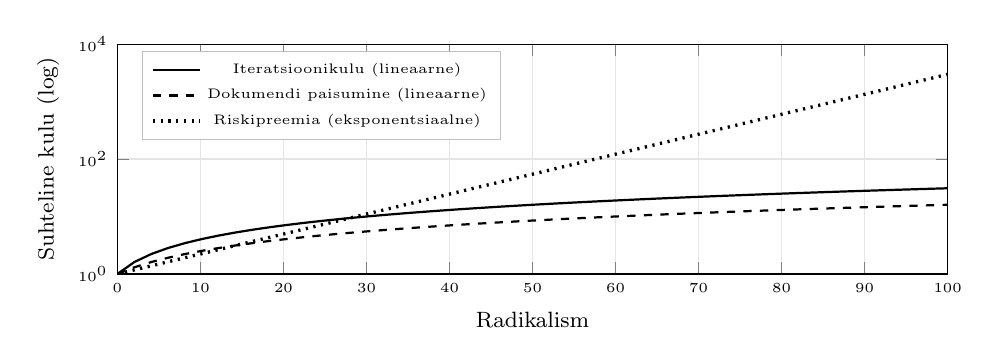
\begin{tikzpicture}
\begin{axis}[
    width=\columnwidth,
    height=4.5cm,
    xlabel={\footnotesize Radikalism},
    ylabel={\footnotesize Suhteline kulu (log)},
    ymode=log,
    xmin=0, xmax=100,
    ymin=1, ymax=10000,
    grid=major,
    grid style={gray!20},
    legend style={at={(0.03,0.97)},anchor=north west,font=\tiny,draw=gray!50},
    tick label style={font=\tiny},
    label style={font=\footnotesize},
]
\addplot[black, thick, domain=0:100, samples=50] {1 + 0.3*x};
\addlegendentry{Iteratsioonikulu (lineaarne)}
\addplot[black, thick, dashed, domain=0:100, samples=50] {1 + 0.15*x};
\addlegendentry{Dokumendi paisumine (lineaarne)}
\addplot[black, thick, dotted, line width=1.2pt, domain=0:100, samples=100] {exp(0.08*x)};
\addlegendentry{Riskipreemia (eksponentsiaalne)}
\end{axis}
\end{tikzpicture}
\caption{Kulude eskaleerumine kolme kanali ulatuses. Riskipreemia domineerib kõrge radikalismi juures.}
\label{fig:radicalism}
\end{figure}

Kriitiline on see, et tegemist ei ole tsensuuriga. Ükski väide ei ole keelatud. Süsteem hinnastab riski (tabel~\ref{tab:costs}).

\begin{table}[ht]
\centering
\caption{Kulude võrdlus väidetüüpide lõikes.}
\label{tab:costs}
\footnotesize
\begin{tabular}{@{}lcccc@{}}
\toprule
\textbf{Tüüp} & \textbf{Iter.} & \textbf{Dok} & \textbf{Tasu} & \textbf{Kokku} \\
\midrule
Usaldusväärne & $k_{\min}$ & $B_0$ & $P_{\min}$ & Madal \\
Vastuoluline & $k_{\text{med}}$ & $B_0{+}k\Delta$ & $\alpha e^{\beta d}$ & Mõõdukas \\
Radikaalne & $k_{\max}$ & $\gg B_0$ & $\gg P_{\min}$ & Väga kõrge \\
Pettuslik & $\to\infty$ & --- & --- & Avaldamatu \\
\bottomrule
\end{tabular}
\end{table}

% ============================================================
% 6. REPUTATION AND RISK
% ============================================================
\section{Reputatsioon ja riskihindamine}

\subsection{Reputatsiooni kogunemise mudel}

Reputatsioonil on kolm omadust: \textbf{aeglane kogunemine} (järkjärguline kasv järjepideva käitumise kaudu), \textbf{kiire hävimine} (üksainus pettus võib skoori katastroofiliselt vähendada) ja \textbf{individuaalne hindamine} (iga tarbiv osapool võib rakendada oma koondamisfunktsiooni).

\subsection{Reputeeritud autoriteedid}

Reputeeritud autoriteet vaatab väited üle ja, kui on rahul, kaasallkirjastab need---pannes kaalule oma reputatsiooni (joonis~\ref{fig:authority}). Asümmeetria on tahtlik: reputatsiooni kogumine on aeglane (järkjärguline $+\delta$ iga ausa kinnitamise kohta), samas kui selle kaotamine on katastroofiline ($-\Delta \gg \delta$ iga vale kinnitamise kohta; illustreerivalt nt $+2\%$ vs.\ $-70\%$). Optimaalne strateegia on alati lükata kahtlased väited tagasi. $\delta$ ja $\Delta$ konkreetsed väärtused on süsteemi parameetrid.

\begin{figure}[ht]
\centering
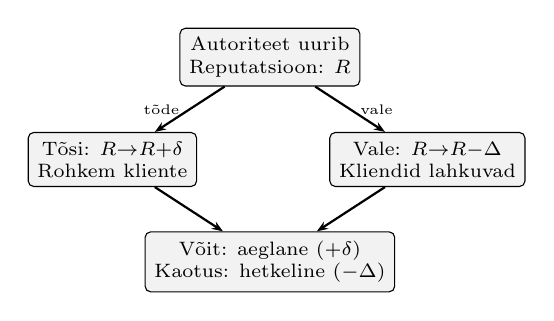
\begin{tikzpicture}[
    box/.style={draw, rounded corners=2pt, minimum width=2cm, minimum height=0.6cm, align=center, font=\scriptsize, fill=black!5},
    arr/.style={-{Stealth[length=4pt]}, thick}
]
\node[box] (exam) at (0,0) {Autoriteet uurib\\Reputatsioon: $R$};
\node[box] (true) at (-2,-1.3) {Tõsi: $R{\to}R{+}\delta$\\Rohkem kliente};
\node[box] (false) at (2,-1.3) {Vale: $R{\to}R{-}\Delta$\\Kliendid lahkuvad};
\node[box] (insight) at (0,-2.6) {Võit: aeglane ($+\delta$)\\Kaotus: hetkeline ($-\Delta$)};

\draw[arr] (exam) -- node[left,font=\tiny] {tõde} (true);
\draw[arr] (exam) -- node[right,font=\tiny] {vale} (false);
\draw[arr] (true) -- (insight);
\draw[arr] (false) -- (insight);
\end{tikzpicture}
\caption{Reputeeritud autoriteet---asümmeetrilised stiimulid.}
\label{fig:authority}
\end{figure}

\subsection{Mitmemõõtmeline reputatsioon}

Reputatsioon ei ole skalaar, vaid vektor mitme mõõtme ulatuses: finantsusaldusväärsus, isiklik ausus, erialane kompetents, kodanikuaktiivsus ja teised (joonis~\ref{fig:reputation-radar}). Erinevad hindamisteenuse pakkujad projitseerivad seda vektorit erinevalt sõltuvalt kontekstist---laenuandja seab esikohale finantsusaldusväärsuse, tööandja erialase kompetentsi, naaber kodanikukäitumise. Puudub üksainus ,,õige'' reputatsiooniskoor; on ainult vaatenurgad.

\begin{figure}[ht]
\centering
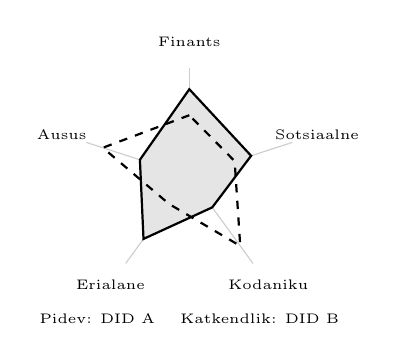
\begin{tikzpicture}[scale=0.55]
\foreach \a/\l in {90/Finants,162/Ausus,234/Erialane,306/Kodaniku,18/Sotsiaalne} {
  \draw[gray!40] (0,0) -- (\a:2.5);
  \node[font=\tiny, align=center] at (\a:3.1) {\l};
  \foreach \r in {0.8,1.6,2.4} {
    \fill[black!15] (\a:\r) circle (0.5pt);
  }
}
\draw[thick, fill=black!10] (90:2.0) -- (162:1.2) -- (234:1.8) -- (306:0.9) -- (18:1.5) -- cycle;
\draw[thick, dashed] (90:1.4) -- (162:2.1) -- (234:0.8) -- (306:2.0) -- (18:1.1) -- cycle;
\node[font=\tiny] at (0,-3.3) {Pidev: DID A \quad Katkendlik: DID B};
\end{tikzpicture}
\caption{Mitmemõõtmelised reputatsioonivektorid. Erinevad DID-id ilmutavad mõõtmete lõikes erinevaid profiile.}
\label{fig:reputation-radar}
\end{figure}

\subsection{Demokratiseeritud riskihindamine}

RSN demokratiseerib süstemaatilise riskihindamise---võimekuse, mis on praegu koondunud finantsasutustesse, kuid mis on rakendatav kaugelt väljaspool pangandust. Tööstuskonglomeraadid, kes hindavad tarnijate usaldusväärsust, kindlustusseltsid, kes hinnastavad käitumuslikku riski, hoolsuskohustus ühinemistel ja ülevõtmistel, seadmete eluea hindamine tootmises---kõikjal, kus vastaspoole riski tuleb hinnata, pakub RSN detsentraliseeritud, turupõhist alternatiivi. Tõlgendusteenuste turg tõlgib toore mitmemõõtmelise reputatsiooniandmestiku tegutsemisvõimelisteks kokkuvõteteks, muutes vastaspoole hindamise kättesaadavaks igale osalejale piirkuluga.

% ============================================================
% 7. CONSENSUS AND DISPUTE RESOLUTION
% ============================================================
\section{Konsensus ja vaidluste lahendamine}

\subsection{Detsentraliseeritud õigluse mudel}

RSN sõnastab õigluse ümber kahepoolse läbirääkimise probleemina. Püsiva, kontrollitava reputatsioonikahju oht on tõhusam heidutus kui kohtumenetlus, mida kahjustatud pool ei suuda endale lubada.

\subsection{Esilekerkiv konsensus}

Iga osaleja säilitab isikliku rahuloluläve. Võrgu koondkonsensus kerkib esile tuhandete kahepoolsete läbirääkimiste statistilise keskmisena (joonis~\ref{fig:consensus}). Konsensusest kaugelt kõrgem vastus (barbaarne) on kallis avaldada. Konsensuse lähedane vastus (proportsionaalne) on odav. Konsensus ei ole reegel---see on hinnasignaal.

\begin{figure}[ht]
\centering
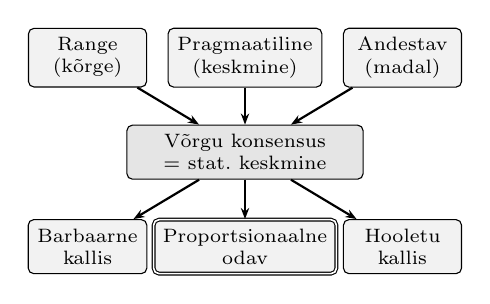
\begin{tikzpicture}[
    person/.style={draw, rounded corners=2pt, minimum width=1.5cm, minimum height=0.5cm, align=center, font=\scriptsize, fill=black!5},
    arr/.style={-{Stealth[length=4pt]}, thick}
]
\node[person] (a) at (-2,0) {Range\\(kõrge)};
\node[person] (b) at (0,0) {Pragmaatiline\\(keskmine)};
\node[person] (c) at (2,0) {Andestav\\(madal)};
\node[person, fill=black!10, minimum width=3cm] (cons) at (0,-1.2) {Võrgu konsensus\\= stat.\ keskmine};
\node[person] (exp) at (-2,-2.4) {Barbaarne\\kallis};
\node[person, double] (prop) at (0,-2.4) {Proportsionaalne\\odav};
\node[person] (neg) at (2,-2.4) {Hooletu\\kallis};

\draw[arr] (a) -- (cons);
\draw[arr] (b) -- (cons);
\draw[arr] (c) -- (cons);
\draw[arr] (cons) -- (exp);
\draw[arr] (cons) -- (prop);
\draw[arr] (cons) -- (neg);
\end{tikzpicture}
\caption{Esilekerkiv konsensus individuaalsetest rahulolulävedest.}
\label{fig:consensus}
\end{figure}

\subsection{Karistuse kalibreerimine}

Iga DID-i valdaja deklareerib avalikult reageeringud konkreetsetele üleastumiskategooriatele. Ebaproportsionaalselt karmid või leebed deklaratsioonid tõmbavad ligi negatiivseid reputatsioonisignaale. Proportsionaalsed deklaratsioonid võetakse vastu hõõrdumiseta---eneseкalibreeruv karistussüsteem.

Konsensusdeklaratsioonid ise alluvad silmakirjalikkuse tuvastamisele: deklaratiivselt konsensuspositsiooni järgimise kohustuse võtmine, käitudes samal ajal ebajärjekindlalt, kujutab endast reputatsioonirikkumist, mis on raskem kui aluseks olev kõrvalekalle, sest see näitab tahtlikku pettust.

\subsection{Delegeerimine}

Kõik tegevused DID-i sees---ühe erandiga---võib delegeerida teisele DID-ile. \textbf{Subjekti roll---DID, kelle käitumisest väide räägib---ei ole delegeeritav; see on mitteülekantavalt seotud identiteedivaldajaga, keda väide puudutab.} Teised aktiivsed rollid---Väljaandja, Autoriteet, Tunnistaja, Kontrollija---saab üle anda määratud delegaat-DID-ile, olgu see kontrollimiseks, väite esitamiseks, konsensuses osalemiseks või vaidluste lahendamiseks. Delegeerimine on igal ajal tühistatav. See võimaldab spetsialiseerumist (nt professionaalsed kontrolliteenused), samal ajal kui valdaja säilitab lõpliku kontrolli ja vastutuse. Delegeerimine kehtib kogu süsteemi ulatuses ja on skaleeritavuse jaoks hädavajalik.

\subsection{Individuaalselt moraalilt esilekerkivale ühiskondlikule lepingule}

Iga DID-i deklareeritud poliitika kujutab endast individuaalse moraali vormistamist: mida valdaja peab vastuvõetavaks, kuidas ta reageerib konkreetsele käitumisele, mida ta nõuab vastaspooltelt. Neid poliitikaid ei kehtesta süsteemi looja---iga osaleja valib need ise ja väljendab neid masinloetaval kujul.

See vormistamine võimaldab kolmeastmelist esilekerkimist. Esiteks kodeeritakse individuaalne moraal \textbf{poliitikana}---deklareeritud reeglite, lävede ja reageeringufunktsioonide kogumina, mida DID kohustub järgima. Teiseks toodab kõigi poliitikate koondsumma kogu võrgu ulatuses \textbf{esilekerkiva eetika}---statistiliselt vaadeldavad normid, mida ükski osaleja ei projekteerinud, kuid mis tekivad tuhandete individuaalsete moraaliseisukohtade interaktsioonist~\cite{durkheim1893}. Kolmandaks moodustavad need esilekerkivad eetikanormid, väljendatuna jagatud käitumuslike normidena, mis on jõustatud kahepoolsete hinnasignaalide kaudu, \textbf{mõõdetava ühiskondliku lepingu}---mitte teoreetilise konstruktsiooni, mille all keegi allkirja pole andnud~\cite{rawls1971}, vaid empiiriliselt vaadeldava reeglistiku, mida toetab tegelik käitumine.

See protsess peegeldab moraalse alusteooria järeldusi~\cite{haidt2012}: inimmoraal on intuitiivne, pluralistlik ja kultuuriliselt varieeruv. RSN ei nõua moraalset konsensust sisendina; see toodab käitumusliku konsensuse väljundina. Sellest tulenev ühiskondlik leping ei ole staatiline---see areneb, kui osalejad liituvad, lahkuvad ja kohandavad oma poliitikaid vastavalt võrgu tagasisidele. Erinevalt klassikalisest ühiskondliku lepingu teooriast on see leping tühistatav, vaadeldav ja jõustatav ilma suverääni.

% ============================================================
% 8. ECONOMIC MODEL
% ============================================================
\section{Majandusmudel}

Eelnevad jaotised kirjeldasid tööriista---RSN-i kontrollimehhanisme, kulustruktuuri ja esilekerkivat konsensust. See jaotis kirjeldab metoodikat selle tööriista rakendamiseks fiskaal- ja valitsemisüleminekule. Tööriist on üldotstarbeline; alljärgnev metoodika on üks võimalik rakendus.

\subsection{Stiimulistruktuur}

Reputatsioon kapitalina loob otsesed stiimulid ausaks käitumiseks. Tavapärases toimimises ehitavad osalejad reputatsiooni loomulikult igapäevaste tehingute ja täidetud kohustuste kaudu. Peamine kulu on \emph{negatiivsetel} väidetel---teiste tekitatud kahju talletamisel. See asümmeetria stimuleerib kasulikku ja usaldusväärset käitumist: aus olemine ei maksa midagi ekstra, samas kui kahjulik olemine loob dokumenteeritud jälje, mille säilitamise eest teised maksavad. Silmakirjalikkus---reeglite deklareerimine ilma neid järgimata---on kõige kallim tõrkerežiim, sest see näitab tahtlikku pettust.

\subsection{Paralleelne fiskaalsüsteem}

Kolm komponenti võimaldavad konkurentsisurvet: (1)~\textbf{Lihtne maks}---üksainus proportsionaalne määr ilma eranditeta, algselt marginaalselt allpool olemasolevat efektiivset määra; (2)~\textbf{Elektrooniline kulutuste registreerimine (ESR)}---Tšehhi EET-mudeli ümberpööramine, nii et kodanikud jälgivad riigi kulutusi; (3)~\textbf{Kodaniku suunatud maksujaotus}---alustades esimesel aastal mõnest protsendist ja jõudes kümnendi järel kusagile madalatest kahekohalistest numbritest kuni täieliku üleminekuni kodaniku suunatud süsteemile, sõltuvalt kasutuselevõtu määrast. Tegelik tempo sõltub kiirusest, millega riigiteenustele tekivad vabaturu alternatiivid, ning riigi valmisolekust üleminekuga koostööd teha; aja funktsioon ei pea olema lineaarne ning puudub põhjus seada ülempiiri sellele, kuhu kasutuselevõtt lõpuks jõuda võib.

% ============================================================
% 9. MIGRATION PATH
% ============================================================
\section{Üleminekutee}

Üleminek toimub kolme faasi kaudu (joonis~\ref{fig:migration}): \textbf{Faas~1: Kate} (RSN informatsioonilise kihina, riik ainus pakkuja), \textbf{Faas~2: Konkurents} (RSN pakub funktsionaalseid alternatiive, kahe süsteemi kasutus) ja \textbf{Faas~3: Üleminek} (RSN edestab riiklikke ekvivalente, vabatahtlik üleminek). Üleminek on pöörduv igas etapis.

\begin{figure}[ht]
\centering
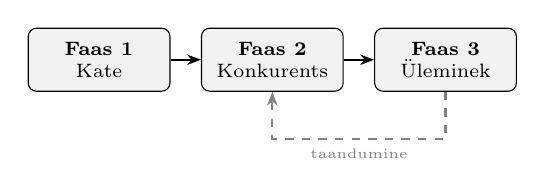
\begin{tikzpicture}[
    phase/.style={draw, rounded corners=3pt, minimum width=1.8cm, minimum height=0.8cm, align=center, font=\scriptsize, fill=black!5},
    arr/.style={-{Stealth[length=5pt]}, thick}
]
\node[phase] (p1) at (0,0) {\textbf{Faas 1}\\Kate};
\node[phase] (p2) at (2.2,0) {\textbf{Faas 2}\\Konkurents};
\node[phase] (p3) at (4.4,0) {\textbf{Faas 3}\\Üleminek};

\draw[arr] (p1) -- (p2);
\draw[arr] (p2) -- (p3);
\draw[arr, dashed, gray] (p3.south) -- ++(0,-0.6) -| node[below,font=\tiny,pos=0.25] {taandumine} (p2.south);
\end{tikzpicture}
\caption{Kolmefaasiline üleminek---pöörduv igas etapis.}
\label{fig:migration}
\end{figure}

Peamine survemehhanism on fiskaalne: kui tingimuslikud maksumaksjad jõuavad ,,majanduslikult olulise vähemuseni $X$''---rühm, mis on piisavalt suur, et repressioon selle vastu põhjustab mittetriviaalset majanduslikku kahju ja kodanikuallumatus muutub usutavaks ohuks---astub riik läbirääkimistesse. Illustratsiooniks kasutame $X \approx 15\%$ SKP-st, kuid tegelik künnis sõltub konkreetsest majandusest.

% ============================================================
% 10. SECURITY ANALYSIS
% ============================================================
\section{Turvaanalüüs}

Vaatleme viit vastasekategooriat: individuaalsed pahatahtlikud tegutsejad, organiseeritud rühmad, ettevõtlusvastased, riigitasandi vastased ja protokollitasandi vastased.

\textbf{Sybil-kindlus}~\cite{douceur2002}. Reputatsiooni ehitamine nõuab püsivat, kontrollitavat interaktsiooni. Eduka Sybil-rünnaku kulu skaleerub lineaarselt võltsidentiteetidega ja ruutsõltuvuses siht-reputatsioonitasemega. Mitme DID-i paralleelne käitamine on võimalik, kuid projekteerituna kulukas---iga identiteet peab reputatsiooni iseseisvalt koguma ehtsa tegevuse kaudu. Vabades ühiskondades heidutab see kulu juhuslikku kuritarvitamist; diktatuurides muutuvad paralleelsed DID-id ellujäämisvahendiks, mis võimaldavad lahterdatud vastupanu, maa-alust koordineerimist ja turvalisemat mustaturu navigeerimist.

\textbf{Kokkumängu kaitse.} Suletud rühmade vastastikuse kinnitamise mustrid on tuvastatavad sotsiaalse graafi analüüsi kaudu. Reputatsiooni koondamise funktsioonid diskonteerivad väiteid tihedalt klasterdunud allikatest.

\textbf{Riigitasandi vastane.} Sibulmarsruutimine, tsentraliseeritud taristu puudumine ja Kontrollija rolli jaotus osalejate baasi ulatuses tagavad, et mahasurumine nõuab meetmeid, mis on ebaproportsionaalsed igasuguse kasuga.

\textbf{Privaatsus vs.\ vastutus.} Pseudonüümsus---kesktee anonüümsuse ja identiteedi avaldamise vahel---võimaldab DID-idel koguda tähendusrikast reputatsiooni ilma valdaja reaalse identiteedi paljastamiseta.

% ============================================================
% 11. PRIVACY
% ============================================================
\section{Privaatsuskaalutlused}

RSN-i privaatsusmudel on üles ehitatud pseudonüümsusele. Valdaja kontrollib identiteedi avaldamist: minimaalne (puhas pseudonüüm), valikuline (konkreetsed tunnistused seotud) või täielik (juriidiline identiteet seotud). Avaldatud väited on püsivad---süsteem toetab kontekstuaalset parandamist, kuid mitte kustutamist. Valdaja võib kompromiteeritud DID-i hüljata ja alustada uuesti, loobudes kogunenud reputatsioonist.

% ============================================================
% 12. RELATED WORK
% ============================================================
\section{Seotud töö}

W3C DID Core spetsifikatsioon~\cite{did2022} ja Ceramic Network~\cite{ceramic2023} pakuvad identiteedi vundamendi. EigenTrust~\cite{kamvar2003} demonstreeris hajutatud reputatsiooni koondamist ilma tsentraalse autoriteedita. SBT-d~\cite{weyl2022} tutvustasid mitteülekantavaid sotsiaalseid märke. RSN erineb oma rõhuasetusega majanduslikule kulule kvaliteedifiltrina ja oma mehhanismiga radikalismi hinnastamiseks.

DAO-d~\cite{buterin2014} ja ruuthääletus~\cite{buterin2019} demonstreerisid detsentraliseeritud valitsemise teostatavust. RSN tuletab konsensuse kahepoolsetest hinnaläbirääkimistest, mitte hääletusest.

Ettepanek toetub anarhokapitalistlikule teooriale~\cite{rothbard1973,hoppe2001} eraviisilise teenusepakkumise osas, kuid lahkneb sellest kahes kriitilises punktis: see on projekteeritud kiuse ja kättemaksuimpulsside jaoks, mitte ei eelda ratsionaalsust, ning see pakub järkjärgulist üleminekut, mitte revolutsiooni. Esilekerkivate ühiskondlike lepingute kontseptsioonil on eelkäijaid Hayeki spontaanse korra teoorias~\cite{hayek1973}.

\textbf{Anarhoagorism.} RSN-il on märkimisväärne ühisosa agoristliku vastumajandusega~\cite{konkin2006}---eelkõige rõhuasetus paralleelsete institutsioonide ehitamisele ja vabatahtlikule vahetusele. Siiski kaldub agorism eeldama ratsionaalset omakasu piisava koordineerimismehhanismina ning sellel puudub sageli konkreetne üleminekutee olemasolevatest riiklikest struktuuridest. RSN hõlmab selgesõnaliselt mitteratsionaalseid käitumuslikke kalduvusi ja pakub fiskaalset survemehhanismi järkjärguliseks üleminekuks.

\textbf{Meritokraatia.} RSN võib kujutada endast esimest funktsionaalset kirjeldust sellest, kuidas meritokraatia~\cite{young1958} saab esile kerkida süsteemse omadusena, mitte loosungina. Traditsioonilised meritokraatlikud süsteemid ebaõnnestuvad, sest need nõuavad tsentraalset autoriteeti ,,teene'' defineerimiseks ja jõustamiseks. RSN-is kerkib teene esile kahepoolsetest hinnangutest: need, kes annavad väärtust, koguvad reputatsiooni; ükski komitee ei otsusta, kellel on teene.

\textbf{Omand kui privileeg.} RSN lahkneb põhimõtteliselt anarhokapitalistlikust ja Austria koolkonna käsitlusest omandiõigustest kui loomulikest ja absoluutsetest. RSN-i raamistikus on omand \emph{privileeg}---sotsiaalne tunnustus, mille kogukond saab äärmuslikel juhtudel tagasi võtta, kui osaleja põhimõtteliselt rikub jagatud norme (reetmine, keeldumine kogukonna kaitsmisest eksistentsiaalses kriisis, süstemaatiline ärakasutamine). See ei ole riiklik sundvõõrandamine, vaid sotsiaalse tunnustuse tagasivõtmine kahepoolsete suhete võrgustiku poolt.

% ============================================================
% 13. LIMITATIONS
% ============================================================
\section{Arutelu ja piirangud}

\textbf{Külmkäivitus.} RSN-i väärtus sõltub võrgumõjudest; varajased kasutuselevõtjad seisavad silmitsi piiratud väärtusega, kuni osalemine saavutab künnise. Siiski, isegi varajastest etappidest alates, on DID-võrk kasulikuks täiendavaks teabeallikaks. Varajase reputatsioonihinnangu ja autoriteedihinnangu eeldatakse arenevat järk-järgult koos kasvava keerukusega.

\textbf{Parasiitluse tõkestamine ja juurdepääsu kontroll.} Siht-DID-id võivad kehtestada astmelisi tasusid ja juurdepääsupiiranguid madala reputatsiooniga DID-ide päringutele. See ei ole binaarne, vaid pidev skaala: mida vähem reputatsiooni päringut esitaval DID-il on, seda vähem teavet ta saab, seda kauem ta ootab ja seda rohkem ta maksab. See mehhanism stimuleerib ehtsat osalust passiivse tarbimise asemel.

\textbf{Juurdepääsu ebavõrdsus.} Väidete avaldamise kulu võib välja filtreerida õiguspärased kaebused majanduslikult ebasoodsas olukorras osalejatelt. Leevendus: iga osaleja tegutseb samaaegselt potentsiaalse kontrollijana (või delegeerib selle rolli) ja teenib kontrollitasusid. Piisava ajahorisondi jooksul peaks mitteradikaalne osaleja lähenema finantsneutraalsusele---kontrollitulu tasakaalustab ligikaudu avaldamiskulud. See on statistiline ootus, mitte garantii.

\textbf{Reputatsiooni ebavõrdsus.} Varajased kasutuselevõtjad koguvad eeliseid, mis võivad luua tõkkeid hilistulnukatele. Siiski teostavad reputatsioonihindamist kolmandast osapoolest pakkujad, kes võivad valida esimese liikuja eelise leevendamise oma koondamisalgoritmide kaudu. Esimesena hea reputatsiooniga olemine on õiguspärane suhteline majanduslik eelis---ja see on tahtlik.

\textbf{Lahtised küsimused.} Optimaalsed kulufunktsioonid, koondamisstandardid, protokolli valitsemine ja interaktsioon AI-genereeritud sünteetiliste reputatsiooniandmetega jäävad tulevase töö valdkondadeks.

See artikkel ei väida, et RSN toodab optimaalseid tulemusi kõikides olukordades. See väidab, et RSN kujutab endast \emph{teostatavat} alternatiivi---tehniliselt rakendatavat, majanduslikult isemajandavat ja sotsiaalselt ühilduvat inimlike käitumuslike kalduvustega sellisena, nagu need tegelikult on.

% ============================================================
% 14. CONCLUSION
% ============================================================
\section{Kokkuvõte}

See artikkel esitas reputatsiooni-suhtlusvõrgustiku, detsentraliseeritud protokolli, mis võimaldab pseudonüümset ja kontrollitavat reputatsioonivahetust. Kalli radikalismi põhimõte tagab, et pettuslikud väited hinnastatakse välja ilma tsensuurita. Väljapakutud üleminekutee võimaldab järkjärgulist ja pöörduvat üleminekut olemasolevatelt institutsioonidelt. Kavand hõlmab inimloomust sellisena, nagu see on---kaasa arvatud väiklus, kius ja kättemaksurahulduse iha---selle asemel, et nõuda ideoloogilist teisenemist. Tulemuseks ei ole utoopia, vaid süsteem, kus õiglus on kättesaadav, reputatsioon on teenitud ja üleastumise kulu kannab pool, kes selle põhjustas.

% ============================================================
% REFERENCES
% ============================================================
\bibliography{references}

\end{document}
